\section{Results for two-dimensional discs}
We first present results from FARGO simulations. The 2D disc spans
$[R_\mathrm{min}, R_\mathrm{max}] = [0.4,10]R_0$. This gives a total
disc mass $M_{d}=0.086M_*$. The mass within
$R\in[R_\mathrm{min},R_{d1}]$ is $0.017M_*$, that within
$R\in[R_{d1},R_{d2}]$ is $0.049M_*$, and that within
$R\in[R_{d2},R_\mathrm{max}]$ is $0.021M_*$. We use a resolution of
$N_R\times N_\phi = 1024\times 2048$, or about $16$ grids per $H$, and
adopt $\epsilon_g=10^{-4}H$ for the   
self-gravity softening length\footnote{In 2D self-gravity, $\epsilon_g$ also
  approximates for the vertical disc thickness, so a more appropriate
  value would be $\epsilon_g\sim H$ \citep{muller12}. However, because
  $\epsilon_g\propto R$ is needed in FARGO, the Poisson kernel
  (Eq. \ref{2d_grav}) is no longer symmetric in $(R,R^\prime)$. We
  choose a small  
  $\epsilon_g$ in favour of angular momentum conservation, keeping in
  mind that the strength of self-gravity will be over-estimated.}.

\subsection{Reference run with random perturbations}
In this fiducial simulation we subject the disc to initial perturbations in
cylindrical radial velocity, 
\begin{align}\label{randpert}
  v_R \to v_R+ c_s\frac{\delta}{M}
  \exp{\left[-\frac{1}{2}\left(\frac{R-\overline{R}_d}{\Delta 
          R_d}\right)^2\right]}\sum_{m=1}^M\cos{m\phi},
\end{align}
where $\delta$ is an amplitude, $\overline{R}_d = (R_{d1}+R_{d2})/2$
and $\Delta R_d = (R_{d2}-R_{d1})/2$. We use $M=10$ and choose 
$\delta\in[-10^{-3},10^{-3}]$ randomly but independent of $\phi$.  

Fig. \ref{fargo_modeamp} plots evolution of the maximum
non-axisymmetric surface density amplitudes in $R\in[R_{d1},R_{d2}]$
for $m\in[1,10]$. Snapshots from the simulation are shown in
Fig. \ref{fargo_2d}. 
At early times $t\lesssim100P_0$ the disc 
dominated by low-amplitude high-$m$ perturbations. The $m\geq4$ modes
growth initially and saturate (or decays) after $t=40P_0$. Notice the
low $m\leq 2$ modes decay initially, but grows between $t\in[20,40]P_0$,
possibily due to saturation of the high-$m$ modes  
\citep{laughlin96,laughlin97}. However, the $m=1$ mode begins to grow
again after $t=70P_0$, and eventually dominates the annulus. 

\begin{figure}
  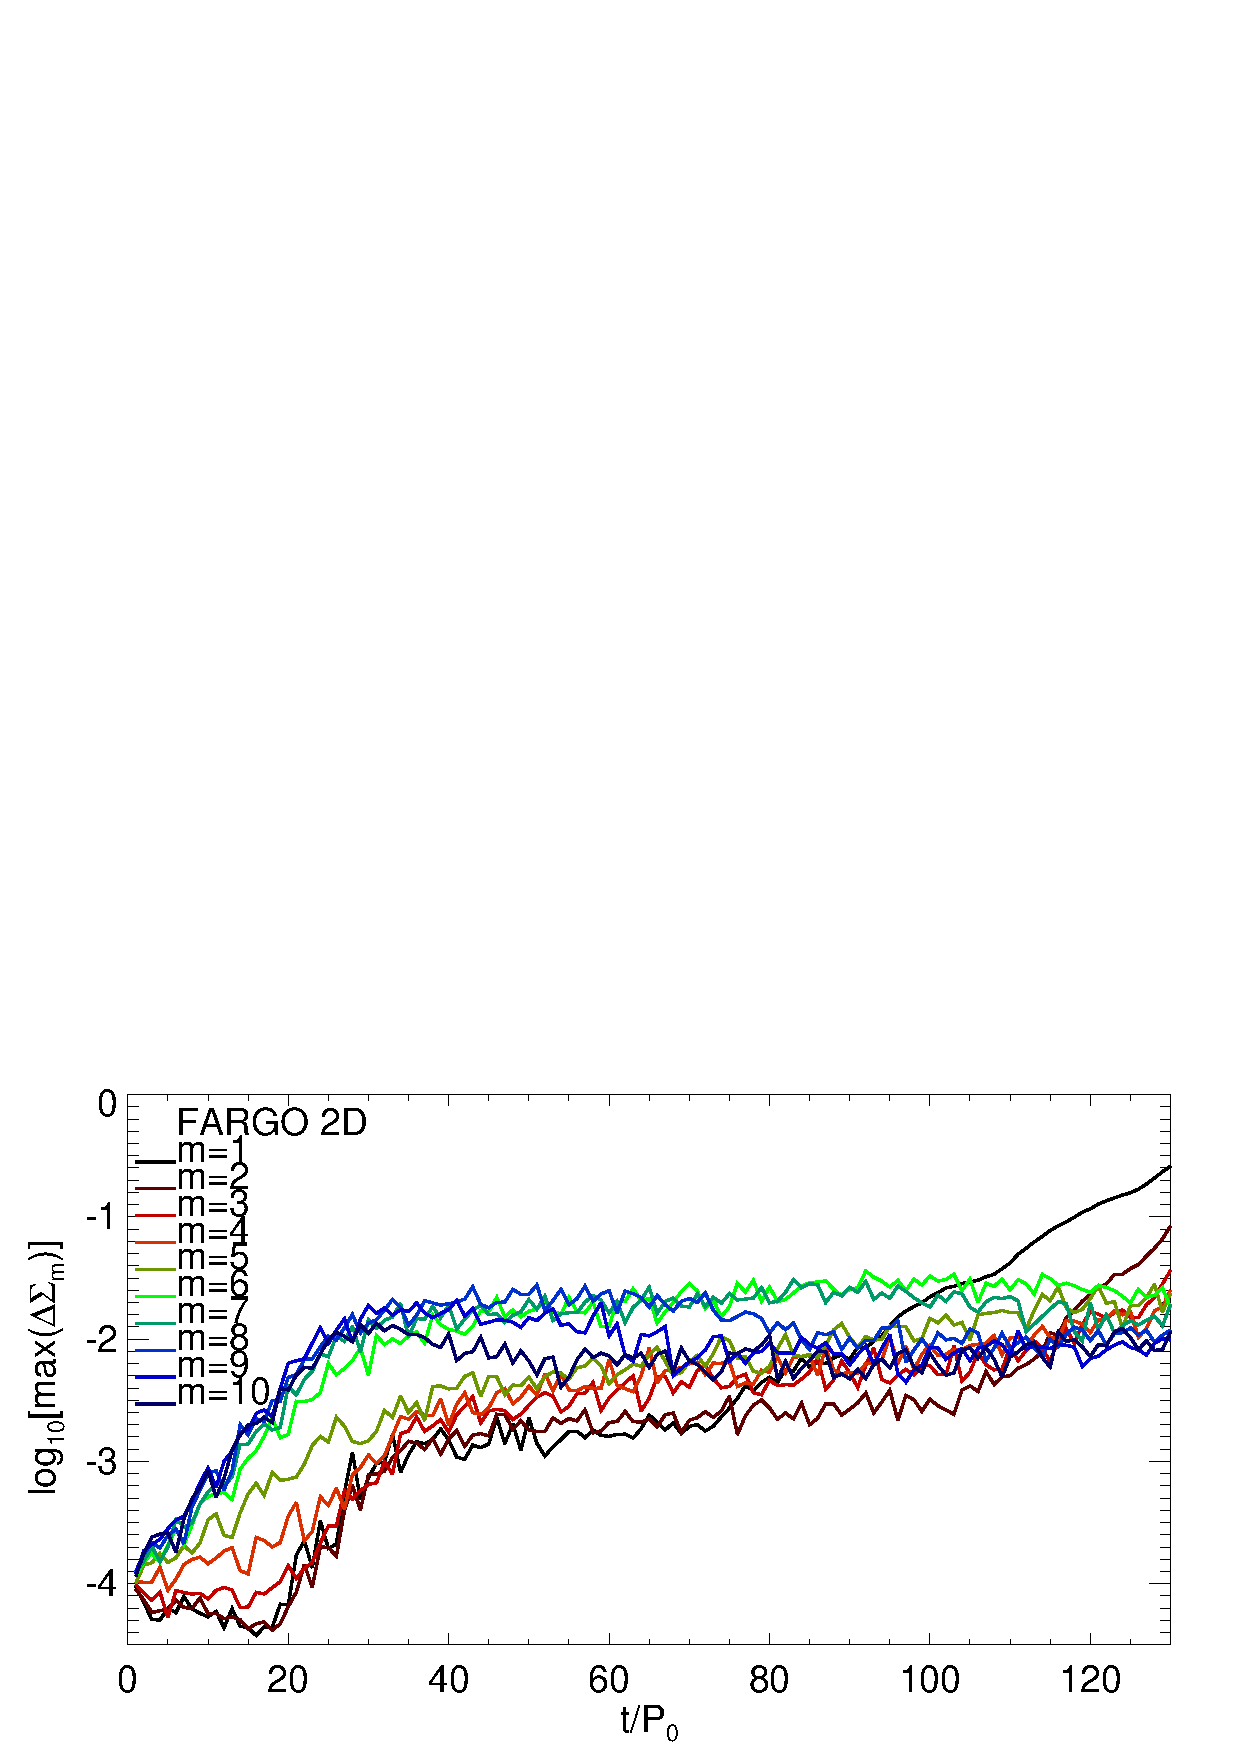
\includegraphics[width=\linewidth]{figures/nonaxi_evol_DZ_fargo}
  \caption{Evolution of maxima in non-axisymmetric surface density 
    in the fiducial FARGO simulation.\label{fargo_modeamp}} 
\end{figure}

\begin{figure}
  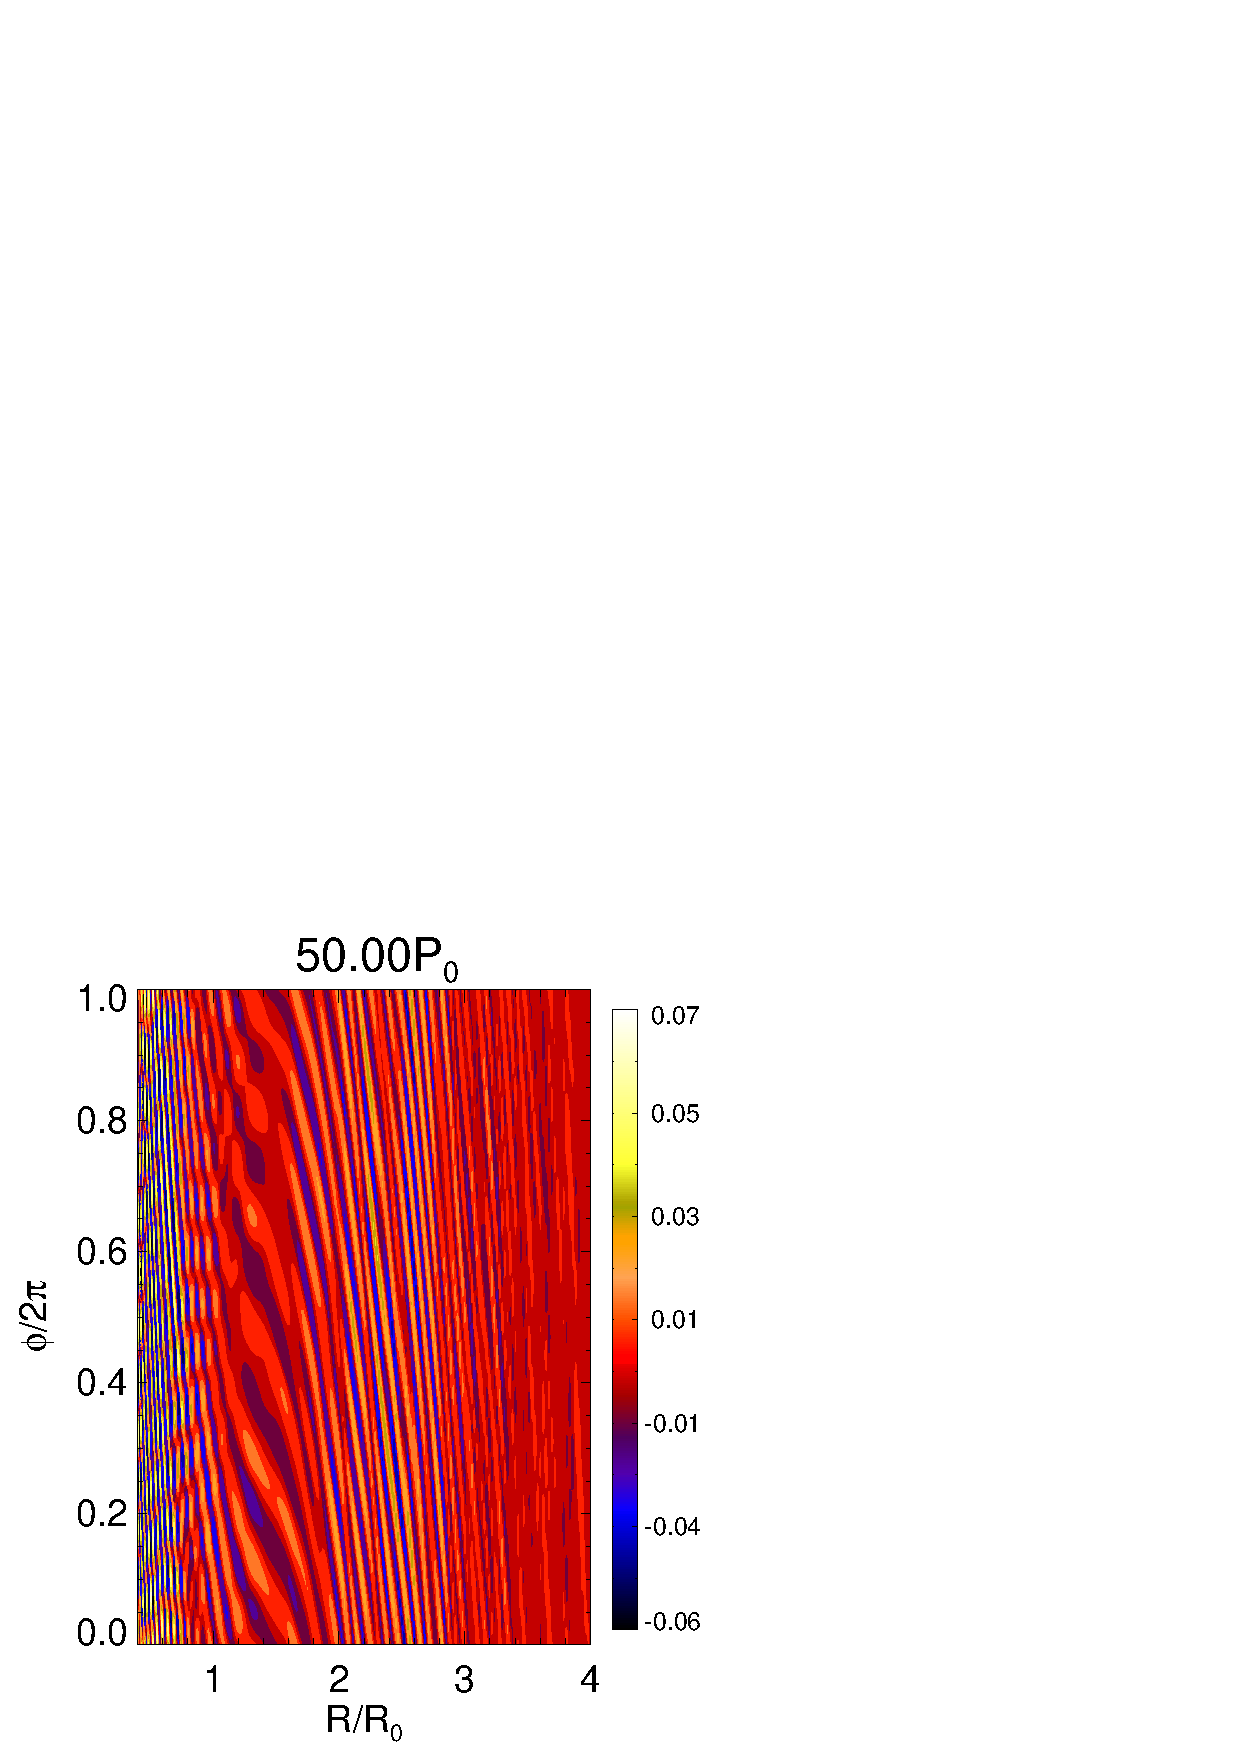
\includegraphics[scale=0.27]{figures/polarxy_dens050}\includegraphics[scale=0.27,clip=true,trim=2.26cm 
  0cm 0cm 
  0cm]{figures/polarxy_dens110}\includegraphics[scale=0.27,clip=true,trim=2.26cm
  0cm 0cm 0cm]{figures/polarxy_dens130} 
  \caption{Visualisation of the FARGO 2D simulation. The total  
    non-axisymmetric surface density
    $\Delta\Sigma$ is shown. \label{fargo_2d}} 
\end{figure}

Fig. \ref{2d_angmom} shows the disc angular momenta
evolution. Only the $m=0,\,1$ components are 
plotted since they are dominant. The $m=1$ structure has
an associated negative angular momentum.   
Its growth is compensated by an increase in the axisymmetric
component of angular momentum, such that $\Delta J_0 + \Delta
J_1 \sim 0$. Note that FARGO does not conserve angular momentum
exactly. However, we find the total angular momentum varies by 
$|\Delta J/J|= O(10^{-6})$, and is much smaller in magnitude than the
change in the angular momenta components, $|\Delta J_{0,1}/J|>
O(10^{-5})$. Fig. \ref{2d_angmom} then suggest that angular momentum
is transferred from the one-arm spiral to the background disc.    

\begin{figure}
  % scale=0.41
  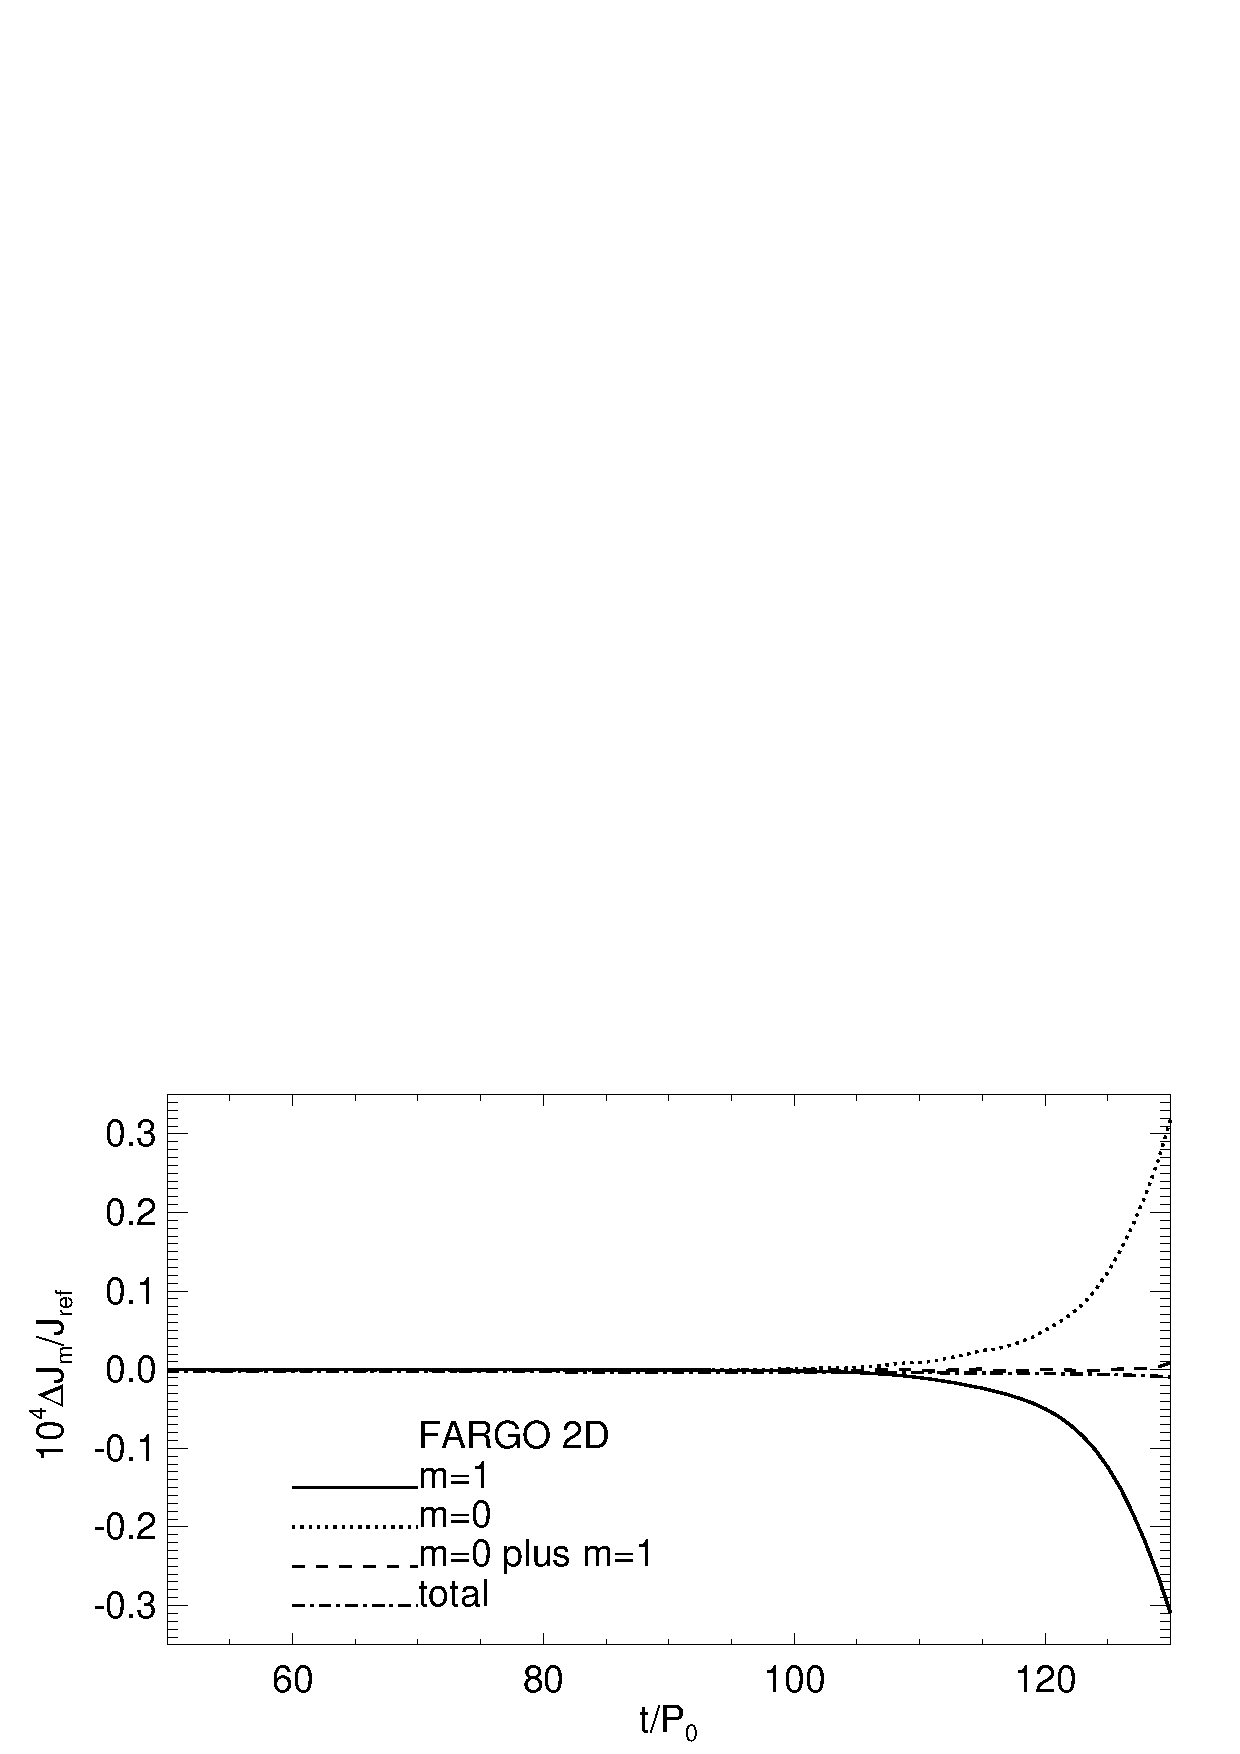
\includegraphics[width=\linewidth]{figures/nonaxi_evol_ang_fargo}
  \caption{Evolution of angular momentum components in the fiducial
    FARGO simulation. The perturbation
    relative to $t=0$ in 2D is shown in units of the
    initial total angular momentum $J_\mathrm{ref}$.\label{2d_angmom}} 
\end{figure}   

\subsection{Trapping the low-frequency $m=1$ spiral}\label{fargo_m1}
In order to focus on the $m=1$ spiral that eventually emerges, here 
we examine a simulation initialised with only $m=1$
perturbations, by setting $M=1$ in Eq. \ref{randpert}. The disc
evolution is largely similar to the previous case, but the final spiral is
more co-herent, facilitating the analysis below. 
Fig. \ref{2d_fargo_viz} shows the $m=1$ surface density
distribution at the end of this simulation.  

\begin{figure}
  \includegraphics[width=\linewidth]{figures/polarxy2_dens120_fargo.ps}
  \caption{Cartesian visualisation of the $m=1$ surface density
    structure in the FARGO simulation initialised with only $m=1$
    perturbations. 
    \label{2d_fargo_viz}} 
\end{figure}   

By examining the disc evolution in $t\in[80,120]P_0$, we find the
one-arm spiral in Fig. \ref{2d_fargo_viz} has a 
co-rotation radius and growth rate of
\begin{align*}
  &R_c \simeq 4.4R_0,\\
  &\gamma\simeq 0.014\Omega_k(R_0) = 0.13\Omega_k(R_c). 
\end{align*}
The spiral can be considered as low frequency because $|\omega|
\lesssim 0.3\Omega$ (recall $\omega = 
m\Omega_p$) in the region it is promininent $R\in[R_{d1},R_{d2}]$. The
growth rate is also slow relative to the local rotation. This gives a
nearly stationary spiral pattern.   

%Since most of
%the perturbation lies at $R<R_c$, this mode has negative
%angular momentum according to local linear theory. 

Next, we write $\Sigma_1 = 
|\Sigma_1|\exp{(\ii kR)}$, where $k$ is real, and assume the amplitude
$|\Sigma_1|$ varies slowly compared to the complex phase. This is the
main assumption in local theory. We plot in
Fig. \ref{fargo_wavenumber} the normalise wavenumber associated with
the $m=1$ spiral. We find that
\begin{align*}
  kR \sim \frac{\pi G \Sigma}{c_s^2}R \sim \frac{1}{hQ}, 
\end{align*}
where we used $Q\sim c_s\Omega/\pi G \Sigma$ and $R\Omega/c_s\sim
h^{-1}$. Since $Q=O(1)$ and $h\ll 1$, $|kR|\gg 1$ and we 
can apply results from local theory self-consistently. Since $k>0$,
the spiral is trailing, as seen in Fig. \ref{2d_fargo_viz}. 

\begin{figure}
  \includegraphics[width=\linewidth]{figures/m1_analysis_kr120_fargo.ps}
  \caption{Normalised radial wavenumber of the $m=1$ spiral in
    Fig. \ref{2d_fargo_viz}.\label{fargo_wavenumber}} 
\end{figure}   

Using the estimated value of $R_c$, we plot in
Fig. \ref{fargo_qbarrier} the quantity $\nu^2 - 1 + Q^{-2}$, which is
required to be positive in local theory for purely wave-like
solutions to the dispersion relation (Eq. \ref{dispersion}) when the
mode frequency is given. The figure shows two $Q$-barriers located in
the inner disc, at $R_{Qb}=R_0$ and $R_{Qb}=1.6R_0$, which is indeed the
region where the $m=1$ spiral develops. This means that the one-arm
spiral is trapped. There is one outer Lindblad resonance at $R_L\simeq
7.2R_0$. Thus, waves may be launched in $R\gtrsim 7.2R_0$ by the main 
spiral disturbance in the inner disc. %this would be a de-stabilising
% effect.  

\begin{figure}
  \includegraphics[width=\linewidth]{figures/m1_analysis_Qbar_fargo.ps} 
  \caption{Dimensionless mode frequency $\nu$ for the $m=1$ spiral in
    Fig. \ref{2d_fargo_viz}. The disperion relation for local density
    waves, Eq. \ref{dispersion}, permits purely wave-like solutions in 
    regions where $\nu^2 - 1 + Q^{-2}>0$. 
    \label{fargo_qbarrier}} 
\end{figure}

\subsection{Angular momentum exchange with the background disc} 
The wavenumber $k = \pi G\Sigma/c_s^2$ corresponds to the
wavelength most susceptible to gravitational instability for
\emph{axisymmetric} perturbations. Physically, then, it is not
surprising to find perturbations of this wavenumber in a
self-gravitating disc where $Q\sim 1$. However, according the
local dispersion relation, $m=1$ perturbations are formally stable for 
real $k$.  

In order to track down the origin for the (slow) growth of the
$m=1$ spiral, we invoke angular momentum conservation for linear
perturbations, Eq. \ref{lin_ang_mom_cons}. Assuming fluxes are
negligible at the disc boundaries, we can integrate
Eq. \ref{lin_ang_mom_cons} to give
\begin{align}\label{baroclinic_torque_int}
  \frac{d}{dt}\underbrace{\int_{R_\mathrm{min}}^{R_\mathrm{max}}\jlin
    2\pi R dR}_{\jlintot} 
  =\int_{R\mathrm{min}}^{R\mathrm{max}}T_\mathrm{BG} 2\pi R dR, 
\end{align}
where we recall $T_{BG}$ is the torque density related to the imposed
sound-speed profile (Eq. \ref{baroclinic_torque}). We have explicitly
computed both sides of Eq. \ref{baroclinic_torque_int} using
simulation data, and compare them in Fig. \ref{fargo_angmom_ex}.  



\begin{figure}
  \includegraphics[width=\linewidth]{figures/m1_analysis_ang_fargo.ps} 
  \caption{
    \label{fargo_angmom_ex}} 
\end{figure}

%ang mom decreases slightly more rapidly than torque exchange provides
%- probably non-linear effects/shocks 